\documentclass[12pt]{article}
\usepackage{amsmath}
\usepackage{graphicx}
\usepackage{hyperref}
\usepackage[latin1]{inputenc}
\usepackage[top=2cm, bottom=2cm, left=2cm, right=2cm, headsep=14pt]{geometry}
\usepackage[T1]{fontenc}
\usepackage[utf8]{inputenc}

\title{Report 2}
\author{Group 2}
%
\date{January 31, 2018}

\begin{document}
\maketitle
  \section{Designing RPC service}
    We use RPCGEN (to generate stubs and runtime program) to communicate between client and server. When the client starts to send message, the stub included in client code receives the request and send it to client runtime program (which will address the server) and then send message to server to execute remote procedure.

    \begin{figure}[h]
        \centering
       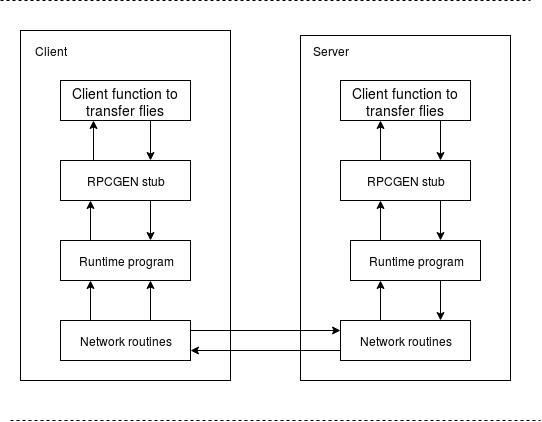
\includegraphics[scale=0.4]{RPC Service.png}
       \caption{RPC service}
    \end{figure}
  
  \section{Organizing the system}
   In client, we write function to read file into a buffer, and we compile it together with RPCGEN code (which allows data to be transferred from client to server and make a remote procedure call). In server, we write function to write data from buffer and compile it with RPCGEN code (which allow us to receive the request from client and execute function). We also create a sample to store struct.
    \begin{figure}[h]
        \centering
       \includegraphics[height=8.35cm]{RPC organize.png}
        \caption{System}
    \end{figure}

  \section{Implementing the file transfer}
    In client, we write function to open file, create a buffer and read file to  \\
    The buffer has 3 attributes: one to store file name, one to store data and one to store number of bytes) \\
    The client then call the remote procedure and send the whole buffer to the server \\
    \begin{verbatim}
    while (1) {
    	/* Read a BLOCK of bytes from file to data. */
        read_bytes = fread(buff.data, 1, BLOCK, file);
        total_bytes += read_bytes;
        buff.numbytes = read_bytes;
        result = filetransfer_proc_1(&buff, cl);
    }
    \end{verbatim}
    A result will show if the process works or not
    \begin{verbatim}
        if (result == NULL) {
            /*An RPC error occurred while calling the server.*/
            clnt_perror(cl, host);
            exit(1);
        }
        /* Successfully called the remote procedure. */
        if (*result == 0) {
            /* A remote system error occurred.*/
            errno = *result;
            perror(name);x`
            exit(1);
        }
    \end{verbatim}
    File data will be read by blocks of 1024 bytes until all the data on server  \\
     \\
    After client receives the remote procedure call from client, server will execute the function to write file (export file) through buffer
    \begin{verbatim}
    file = fopen(recvbuff->name, "a");
    if (file == NULL) {
        write_bytes = -1;
        return &write_bytes;
    }
    write_bytes = fwrite(recvbuff->data, 1, recvbuff->numbytes, file);
    fclose(file);
    \end{verbatim}
 
\end{document}